\chapter{Cameras}
\label{ch:cameras}

The observation model $h(\x_k,\m_j)$ of Chapter~\ref{ch:slam} is, for a
camera, a composition of three maps: a rigid motion that brings the
landmark into the camera frame, a perspective division that throws away
its depth, and a lens-and-sensor map that turns the result into a pixel.
This chapter makes each map precise, differentiates the composition (the
Jacobians every later chapter needs), shows how the unknown parameters of
the lens and sensor are estimated from images of a checkerboard, and
explains what a second camera buys: depth, with an uncertainty that grows
with its square.

\section{The pinhole model}

\begin{definition}{Camera frame and normalised coordinates}{camframe}
The \emph{camera frame} has its origin at the optical centre, its $z$
axis along the optical axis pointing into the scene, its $x$ axis to the
right and its $y$ axis down in the image (the OpenCV convention). A point
$\vect{q}=(X,Y,Z)\T$ with $Z>0$ in this frame has \emph{normalised
coordinates}
\[
\vect{x}=\pi(\vect{q})=\Bigl(\frac{X}{Z},\ \frac{Y}{Z}\Bigr)\T,
\]
its intersection with the plane $Z=1$.
\end{definition}

A physical camera with focal length $f$ forms the image on the plane
$Z=f$, so by similar triangles the image of $\vect{q}$ sits at
$f\vect{x}$ in metric units. The sensor samples that plane with pixels of
size $\rho_u\times\rho_v$, and pixel $(0,0)$ is in a corner, not on the
optical axis. Hence:

\begin{definition}{Intrinsic matrix}{intrinsics}
The pixel coordinates of $\vect{q}$ are $\vect{u}=(u,v)\T$ with
\[
\begin{pmatrix}u\\v\\1\end{pmatrix}=K\begin{pmatrix}x\\y\\1
\end{pmatrix},\qquad
K=\begin{pmatrix}f_x&s&c_x\\0&f_y&c_y\\0&0&1\end{pmatrix},
\]
where $f_x=f/\rho_u$ and $f_y=f/\rho_v$ are the focal lengths in pixels,
$(c_x,c_y)$ is the \emph{principal point} (where the optical axis meets
the sensor) and $s$ is a skew, zero for every modern sensor.
\end{definition}

\subsection{Homogeneous coordinates and the projection matrix}

\begin{definition}{Projective plane}{p2}
Two nonzero vectors $\tilde{\vect{u}},\tilde{\vect{u}}'\in\R^3$ are
\emph{equivalent}, $\tilde{\vect{u}}\sim\tilde{\vect{u}}'$, if
$\tilde{\vect{u}}'=\lambda\tilde{\vect{u}}$ for some $\lambda\neq0$. The
projective plane $\mathbb{P}^2$ is the set of equivalence classes. A point
$\vect{u}\in\R^2$ is represented by $\tilde{\vect{u}}=(\vect{u},1)$, and a
class with third coordinate $w\neq0$ represents the point
$(\tilde u_1/w,\tilde u_2/w)$.
\end{definition}

\begin{proposition}{The projection matrix}{projmat}
Let the camera have pose $T_{wc}=(R_{wc},\vect{c})$, so that its centre
is $\vect{c}$ in the world frame, and write $T_{cw}=T_{wc}^{-1}=
(R_{cw},\vect{t}_{cw})$. Ignoring lens distortion, a world point
$\p_w$ in front of the camera projects to
\begin{equation}\label{eq:projmat}
\tilde{\vect{u}}\sim P\tilde{\p}_w,\qquad
P=K\,[\,R_{cw}\ \ \vect{t}_{cw}\,]\in\R^{3\times4}.
\end{equation}
\end{proposition}

\begin{proof}
$\vect{q}=R_{cw}\p_w+\vect{t}_{cw}=[\,R_{cw}\ \vect{t}_{cw}\,]\tilde\p_w$
and $(\vect{x},1)=\vect{q}/Z$, so $(\vect{u},1)=K\vect{q}/Z\sim
K\vect{q}$.
\end{proof}

\begin{lemma}{The ray of a pixel}{ray}
The points of $\R^3$ in front of the camera that project to the pixel
$\vect{u}$ form the open ray
$\{\vect{c}+\lambda R_{wc}K^{-1}\tilde{\vect{u}}:\lambda>0\}$.
\end{lemma}

\begin{proof}
$\p_w$ projects to $\vect{u}$ if and only if $\vect{q}=T_{cw}\p_w$
satisfies $K\vect{q}=Z\tilde{\vect{u}}$ with $Z>0$, i.e.\
$\vect{q}=Z K^{-1}\tilde{\vect{u}}$ ($K$ is invertible since
$f_x,f_y>0$). Mapping back to the world, $\p_w=R_{wc}\vect{q}+\vect{c}$.
\end{proof}

\begin{inwords}
A camera measures \emph{directions}, not points. Everything on the ray
through the optical centre and the pixel produces the same image. Depth
must come from elsewhere: from a second view taken from another place
(triangulation, Chapter~6), from a second camera (stereo, below), or
from a motion sensor (Part~IV). This is the monocular scale gauge of
Chapter~\ref{ch:slam} seen from the sensor's side.
\end{inwords}

\section{Lens distortion}

Real lenses, especially the wide-angle ones that make visual tracking
robust, bend straight lines. The standard model acts on normalised
coordinates, between $\pi$ and $K$.

\begin{definition}{Radial--tangential distortion}{distortion}
With $r^2=x^2+y^2$ and coefficients $(k_1,k_2,p_1,p_2,k_3)$, the
distortion map $d:\vect{x}\mapsto\vect{x}_d$ is
\begin{align*}
x_d&=x\,\rho(r^2)+2p_1xy+p_2(r^2+2x^2),\\
y_d&=y\,\rho(r^2)+p_1(r^2+2y^2)+2p_2xy,\qquad
\rho(r^2)=1+k_1r^2+k_2r^4+k_3r^6 .
\end{align*}
The full projection is then $\vect{u}=\kappa(d(\pi(\vect{q})))$ with the
affine map $\kappa(\vect{x}_d)=(f_xx_d+c_x,\ f_yy_d+c_y)$.
\end{definition}

The radial term models the lens shape: $k_1<0$ is \emph{barrel}
distortion, typical of wide-angle lenses, where points are pulled
towards the centre more strongly the further out they are
(\cref{fig:distortion}). The tangential terms $p_1,p_2$ model a lens that
is slightly decentred or tilted with respect to the sensor. For fisheye
lenses with fields of view near or beyond $180^\circ$ this polynomial
model breaks down, and one uses instead a model in the angle $\theta$
between the ray and the optical axis, such as the equidistant model
$r_d=\theta(1+k_1\theta^2+k_2\theta^4+\cdots)$.

\begin{proposition}{Undistortion is well posed near the centre}{undistort}
The Jacobian of $d$ at $\vect{x}$ is
\[
\frac{\partial\vect{x}_d}{\partial\vect{x}}=
\begin{pmatrix}
\rho+gx^2+2p_1y+6p_2x & gxy+2p_1x+2p_2y\\
gxy+2p_1x+2p_2y & \rho+gy^2+6p_1y+2p_2x
\end{pmatrix},\qquad g=2k_1+4k_2r^2+6k_3r^4 .
\]
It equals $I$ at $\vect{x}=\vect0$, so $d$ is a diffeomorphism from a
neighbourhood of $\vect0$ onto a neighbourhood of $\vect0$, and Newton's
iteration $\vect{x}\leftarrow\vect{x}-(\partial d/\partial\vect{x})^{-1}
(d(\vect{x})-\vect{x}_d)$ started at $\vect{x}=\vect{x}_d$ converges
quadratically to $d^{-1}(\vect{x}_d)$ when $\vect{x}_d$ is close enough
to $\vect0$.
\end{proposition}

\begin{proof}
Write $\rho'=\mathrm{d}\rho/\mathrm{d}(r^2)=k_1+2k_2r^2+3k_3r^4$. Then
$\partial\rho/\partial x=2x\rho'=gx$ and $\partial\rho/\partial y=gy$.
Differentiating the definition term by term,
$\partial x_d/\partial x=\rho+x\cdot gx+2p_1y+p_2(2x+4x)$,
$\partial x_d/\partial y=x\cdot gy+2p_1x+2p_2y$, and symmetrically for
$y_d$. At $\vect{x}=\vect0$, $\rho=1$ and every other term vanishes. The
inverse function theorem gives the local diffeomorphism, and the standard
local convergence theorem for Newton's method (a $C^2$ map with
invertible Jacobian at the root) gives quadratic convergence from close
enough starting points; $\vect{x}_d$ is such a point because
$d(\vect{x})=\vect{x}+O(\norm{\vect{x}}^3)$ near the centre.
\end{proof}

Far from the centre the model can fold back on itself (the radial map
$r\mapsto r\rho(r^2)$ stops being monotonic), and it is then meaningless.
Calibration only constrains it where the target was seen, so one never
trusts it outside the calibrated field of view.

\begin{figure}[ht]
\centering
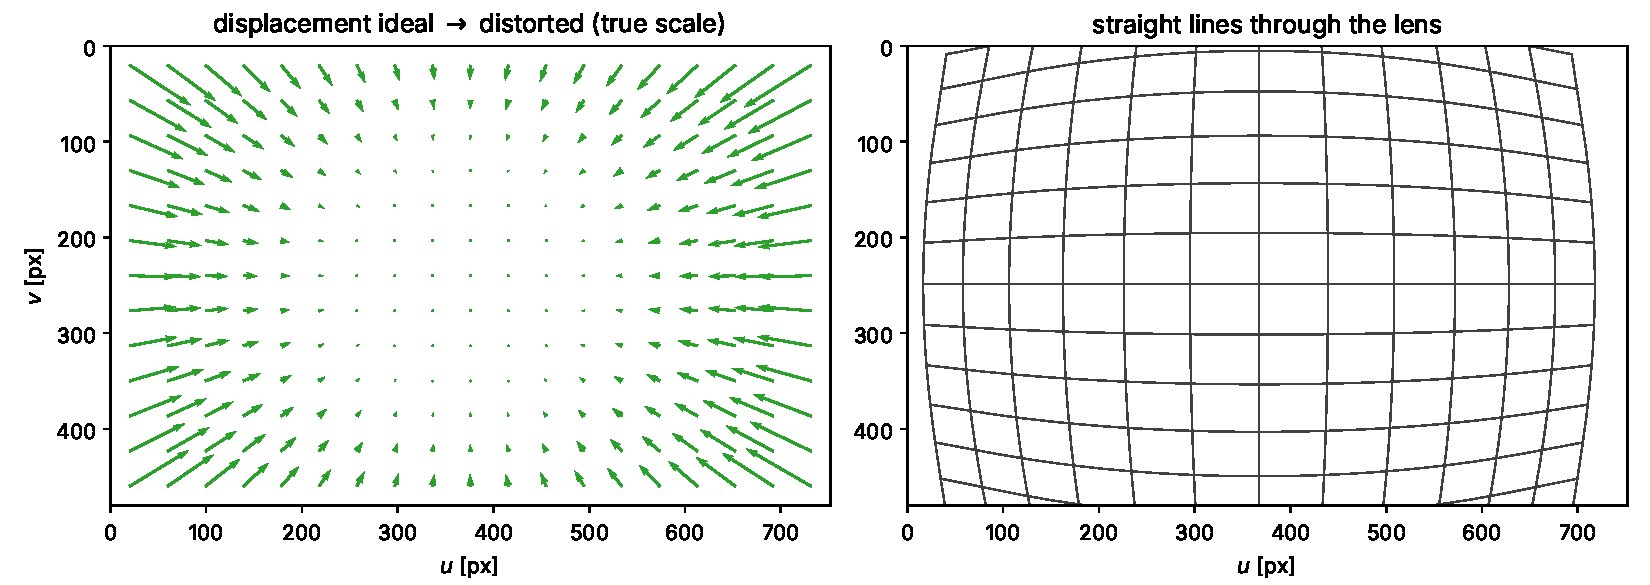
\includegraphics[width=\linewidth]{figures/ch03_distortion.pdf}
\caption{A wide-angle lens ($k_1=-0.28$, $k_2=0.07$). Left: where each
ideal pixel is moved to, at true scale; near the corners the shift
exceeds 40 pixels. Right: the image of a square grid of straight lines.}
\label{fig:distortion}
\end{figure}

\section{The reprojection Jacobians}

Every visual residual in this course has the form
$\vect{e}=\z-\vect{u}(T_{wc},\p_w)$. Its Jacobians follow from the chain
rule and Exercise~\ref{ex:2cam}.

\begin{proposition}{Jacobians of the projection}{projjac}
Let $\vect{q}=T_{wc}^{-1}\p_w=(X,Y,Z)$ and $\vect{u}=\kappa(d(\pi(
\vect{q})))$. With a right perturbation $\bxi=(\brho,\bphi)$ of $T_{wc}$,
\[
\frac{\partial\vect{u}}{\partial\bxi}=F\,D\,\Pi\,
[\,-I\ \ \hatop{\vect{q}}\,],\qquad
\frac{\partial\vect{u}}{\partial\p_w}=F\,D\,\Pi\,R_{wc}\T,
\]
where $F=\diag(f_x,f_y)$, $D=\partial\vect{x}_d/\partial\vect{x}$ from
\cref{prop:undistort} and
\[
\Pi=\frac{\partial\pi}{\partial\vect{q}}=\begin{pmatrix}1/Z&0&-X/Z^2\\
0&1/Z&-Y/Z^2\end{pmatrix}.
\]
Without distortion ($D=I$), with $x=X/Z$ and $y=Y/Z$,
\begin{equation}\label{eq:projjac}
\frac{\partial\vect{u}}{\partial\bxi}=\begin{pmatrix}
-\dfrac{f_x}{Z}&0&\dfrac{f_xx}{Z}&f_xxy&-f_x(1+x^2)&f_xy\\[2mm]
0&-\dfrac{f_y}{Z}&\dfrac{f_yy}{Z}&f_y(1+y^2)&-f_yxy&-f_yx
\end{pmatrix}.
\end{equation}
\end{proposition}

\begin{proof}
The chain rule through $\vect{u}=\kappa\circ d\circ\pi$ gives the factor
$FD\Pi$; $\partial\vect{q}/\partial\bxi=[\,-I\ \hatop{\vect{q}}\,]$ and
$\partial\vect{q}/\partial\p_w=R_{wc}\T$ are Exercise~\ref{ex:2cam}.
For \eqref{eq:projjac}, $\Pi(-I)=\bigl(\begin{smallmatrix}-1/Z&0&x/Z\\
0&-1/Z&y/Z\end{smallmatrix}\bigr)$, and with $\hatop{\vect{q}}=
\bigl(\begin{smallmatrix}0&-Z&Y\\Z&0&-X\\-Y&X&0\end{smallmatrix}\bigr)$,
the first row of $\Pi\hatop{\vect{q}}$ is
$\frac1Z(0,-Z,Y)-\frac{X}{Z^2}(-Y,X,0)=(xy,\,-(1+x^2),\,y)$ and the
second is $\frac1Z(Z,0,-X)-\frac{Y}{Z^2}(-Y,X,0)=(1+y^2,\,-xy,\,-x)$.
Multiply by $F$.
\end{proof}

\begin{inwords}
Read \eqref{eq:projjac} column by column. Translating the camera
sideways by $\rho_1$ moves the pixel by $-f_x\rho_1/Z$: near points move
a lot, far points barely move, which is why distant features constrain
rotation well and translation poorly. Rotating the camera (last three
columns) moves every pixel by an amount that does \emph{not} depend on
$Z$: rotation is observable from any feature, near or far. On an open
lawn, where the stable features (trees, the house) are far away, the
mower's heading will be well constrained by vision and its position much
less so.
\end{inwords}

\section{Calibration from a planar target}

We now estimate $K$ (and later the distortion) from images of a
checkerboard whose corners are at known positions $(X_i,Y_i,0)$ in a
\emph{board frame} $b$. Let $T_{cb}=(R,\vect{t})$ be the pose of the
board in the camera frame, and $\vect{r}_1,\vect{r}_2,\vect{r}_3$ the
columns of $R$.

\begin{definition}{Homography}{homography}
A \emph{homography} is an invertible map of $\mathbb{P}^2$ given by an
invertible $3\times3$ matrix $H$, defined up to scale:
$\tilde{\vect{u}}\mapsto H\tilde{\vect{u}}$.
\end{definition}

\begin{lemma}{The board-to-image homography}{boardH}
Ignoring distortion, the corner $(X,Y,0)$ projects to
$\tilde{\vect{u}}\sim H(X,Y,1)\T$ with
$H\sim K[\,\vect{r}_1\ \ \vect{r}_2\ \ \vect{t}\,]$.
\end{lemma}

\begin{proof}
By \cref{prop:projmat}, $\tilde{\vect{u}}\sim K[\,R\ \vect{t}\,](X,Y,0,
1)\T=K(X\vect{r}_1+Y\vect{r}_2+\vect{t})$. The matrix is invertible
because the camera centre is not on the board plane.
\end{proof}

\subsection{Estimating a homography}

\begin{proposition}{Direct linear transform}{dlt}
Let $\vect{h}\in\R^9$ stack the rows $\vect{h}^{1\mathsf T},
\vect{h}^{2\mathsf T},\vect{h}^{3\mathsf T}$ of $H$. A correspondence
$\vect{p}=(X,Y,1)\T\mapsto(u,v)$ gives two linear equations
\[
\begin{pmatrix}\vect0\T&-\vect{p}\T&v\,\vect{p}\T\\
\vect{p}\T&\vect0\T&-u\,\vect{p}\T\end{pmatrix}\vect{h}=\vect0 .
\]
Stacking $N\ge4$ correspondences gives $A\vect{h}=\vect0$ with
$A\in\R^{2N\times9}$. The minimiser of $\norm{A\vect{h}}$ subject to
$\norm{\vect{h}}=1$ is the right singular vector of $A$ for its smallest
singular value.
\end{proposition}

\begin{proof}
$\tilde{\vect{u}}\sim H\vect{p}$ is equivalent to
$\tilde{\vect{u}}\times H\vect{p}=\vect0$ with $\tilde{\vect{u}}=
(u,v,1)$. Since $H\vect{p}=(\vect{h}^{1\mathsf T}\vect{p},
\vect{h}^{2\mathsf T}\vect{p},\vect{h}^{3\mathsf T}\vect{p})$, the first
two components of the cross product are
$v\,\vect{h}^{3\mathsf T}\vect{p}-\vect{h}^{2\mathsf T}\vect{p}$ and
$\vect{h}^{1\mathsf T}\vect{p}-u\,\vect{h}^{3\mathsf T}\vect{p}$, the
two rows above; the third is a linear combination of them. For the
minimisation, let $A=U\Sigma V\T$ be an SVD with singular values
$\sigma_1\ge\dots\ge\sigma_9\ge0$ and columns $\vect{v}_i$ of $V$. For
$\norm{\vect{h}}=1$, write $\vect{h}=\sum_i\alpha_i\vect{v}_i$ with
$\sum\alpha_i^2=1$; then $\norm{A\vect{h}}^2=\vect{h}\T V\Sigma\T\Sigma
V\T\vect{h}=\sum_i\sigma_i^2\alpha_i^2\ge\sigma_9^2$, with equality for
$\vect{h}=\vect{v}_9$.
\end{proof}

The quantity minimised is an \emph{algebraic} error, not a distance in
pixels, and its value depends on the coordinate system: pixel
coordinates in the hundreds next to the constant $1$ make $A$ badly
conditioned. Hartley's remedy is to first apply similarities
$T$, $T'$ that move each point set's centroid to the origin and scale it
to mean distance $\sqrt2$, estimate $\hat H$ between the normalised
sets, and return $H=T'^{-1}\hat HT$. This is exact (if $\hat{\tilde
{\vect{u}}}=T'\tilde{\vect{u}}$, $\hat{\vect{p}}=T\vect{p}$ and
$\hat{\tilde{\vect{u}}}\sim\hat H\hat{\vect{p}}$, then $\tilde{\vect{u}}
\sim T'^{-1}\hat HT\vect{p}$), costs nothing, and is never optional.

\subsection{Zhang's method}

\begin{theorem}{Zhang's constraints}{zhang}
Let $\vect{h}_1,\vect{h}_2$ be the first two columns of a board
homography $H$ and $B=K^{-\mathsf T}K^{-1}$. Then
\begin{equation}\label{eq:zhang}
\vect{h}_1\T B\,\vect{h}_2=0,\qquad
\vect{h}_1\T B\,\vect{h}_1=\vect{h}_2\T B\,\vect{h}_2 .
\end{equation}
These are linear in the six distinct entries
$\vect{b}=(B_{11},B_{12},B_{22},B_{13},B_{23},B_{33})$ of the symmetric
matrix $B$.
\end{theorem}

\begin{proof}
By \cref{lem:boardH}, $H=\mu K[\,\vect{r}_1\ \vect{r}_2\ \vect{t}\,]$ for
some $\mu\neq0$, so $K^{-1}\vect{h}_i=\mu\vect{r}_i$ for $i=1,2$. Hence
$\vect{h}_i\T B\vect{h}_j=(K^{-1}\vect{h}_i)\T(K^{-1}\vect{h}_j)=
\mu^2\,\vect{r}_i\T\vect{r}_j$. The columns of a rotation are
orthonormal: $\vect{r}_1\T\vect{r}_2=0$ and
$\vect{r}_1\T\vect{r}_1=\vect{r}_2\T\vect{r}_2=1$. Linearity in
$\vect{b}$: $\vect{a}\T B\vect{c}=\sum_{k,l}B_{kl}a_kc_l$, and grouping
the symmetric pairs gives $\vect{v}(\vect{a},\vect{c})\T\vect{b}$ with
$\vect{v}=(a_1c_1,\ a_1c_2+a_2c_1,\ a_2c_2,\ a_3c_1+a_1c_3,\
a_3c_2+a_2c_3,\ a_3c_3)$.
\end{proof}

\begin{inwords}
$B$ (the ``image of the absolute conic'') is the metric that the
intrinsics induce on image directions: $\tilde{\vect{u}}\T B\,
\tilde{\vect{u}}'$ is, up to scale, the inner product of the two
viewing rays. Each view of a plane shows two directions (the board's
$X$ and $Y$ axes) that we \emph{know} are orthogonal and equally scaled,
and that knowledge pins down $B$, hence $K$.
\end{inwords}

Each view gives two equations; $\vect{b}$ has six entries but is only
defined up to scale, so it has five degrees of freedom and \emph{three
views in general position} suffice. If the skew is known to be zero we
may add the equation $B_{12}=0$ (Exercise~\ref{ex:3skew}), and two views
suffice. With $n$ views, stack the $2n$ equations into $V\vect{b}=\vect0$
and take the singular vector of \cref{prop:dlt}.

\begin{proposition}{Recovering $K$ from $B$}{kfromb}
Let $\hat B=\mu K^{-\mathsf T}K^{-1}$ be the estimate, $\mu\neq0$
unknown. Replace $\hat B$ by $-\hat B$ if $\hat B_{11}<0$. Then
$\hat B\succ0$, its Cholesky factorisation $\hat B=LL\T$ satisfies
$L=\sqrt{\mu}\,K^{-\mathsf T}$, and $K$ is $(L\T)^{-1}$ divided by its
$(3,3)$ entry.
\end{proposition}

\begin{proof}
$K^{-\mathsf T}K^{-1}=(K^{-1})\T K^{-1}$ is positive definite since
$K^{-1}$ is invertible, so $\hat B$ is definite with the sign of $\mu$,
and the sign of $\hat B_{11}$ reveals it. After the sign change $\mu>0$.
$K$ is upper triangular with positive diagonal $(f_x,f_y,1)$, hence so
is $K^{-1}$, and $K^{-\mathsf T}$ is lower triangular with positive
diagonal. So $\sqrt\mu K^{-\mathsf T}$ is a lower-triangular matrix with
positive diagonal whose product with its transpose is $\hat B$; by
uniqueness of the Cholesky factor it is $L$. Then $(L\T)^{-1}=K/
\sqrt\mu$, and dividing by the $(3,3)$ entry $1/\sqrt\mu$ gives $K$.
\end{proof}

Once $K$ is known, each view's pose follows from \cref{lem:boardH}:
$\vect{r}_i=\lambda K^{-1}\vect{h}_i$ with $\lambda=1/\norm{K^{-1}
\vect{h}_1}$, $\vect{t}=\lambda K^{-1}\vect{h}_3$, $\vect{r}_3=
\vect{r}_1\times\vect{r}_2$, the sign of $\lambda$ chosen so that
$t_z>0$ (the board is in front of the camera). With noise the matrix
$M=[\,\vect{r}_1\ \vect{r}_2\ \vect{r}_3\,]$ is not exactly a rotation,
and we replace it by the nearest one.

\begin{lemma}{Nearest rotation}{nearestrot}
Let $M=U\Sigma V\T$ be an SVD. If $\det(UV\T)=1$, the rotation
minimising $\norm{R-M}_F$ is $R^\star=UV\T$. In general it is
$U\diag(1,1,\det(UV\T))V\T$.
\end{lemma}

\begin{proof}
$\norm{R-M}_F^2=\norm{R}_F^2+\norm{M}_F^2-2\tr(R\T M)=3+\norm{M}_F^2-2\tr
(R\T M)$, so we maximise $\tr(R\T M)=\tr(\Sigma\,W)$ with
$W=V\T R\T U$, an orthogonal matrix. Its entries satisfy $|W_{ii}|\le1$,
so $\tr(\Sigma W)=\sum_i\sigma_iW_{ii}\le\sum_i\sigma_i$, with equality
when $W=I$, i.e.\ $R=UV\T$; this $R$ is admissible exactly when
$\det(UV\T)=1$. When $\det(UV\T)=-1$, admissible $W$ have
$\det W=-1$, and the maximum $\sigma_1+\sigma_2-\sigma_3$ is attained at
$W=\diag(1,1,-1)$; we do not prove this case here (see Umeyama, 1991).
\end{proof}

The linear step ignores distortion and minimises algebraic, not pixel,
errors. It is an \emph{initialisation}: the final calibration minimises
the reprojection error over $K$, the distortion and all board poses
together, by the nonlinear least squares of Chapter~4. This is exactly
what OpenCV's \code{calibrateCamera} does.

\begin{figure}[ht]
\centering
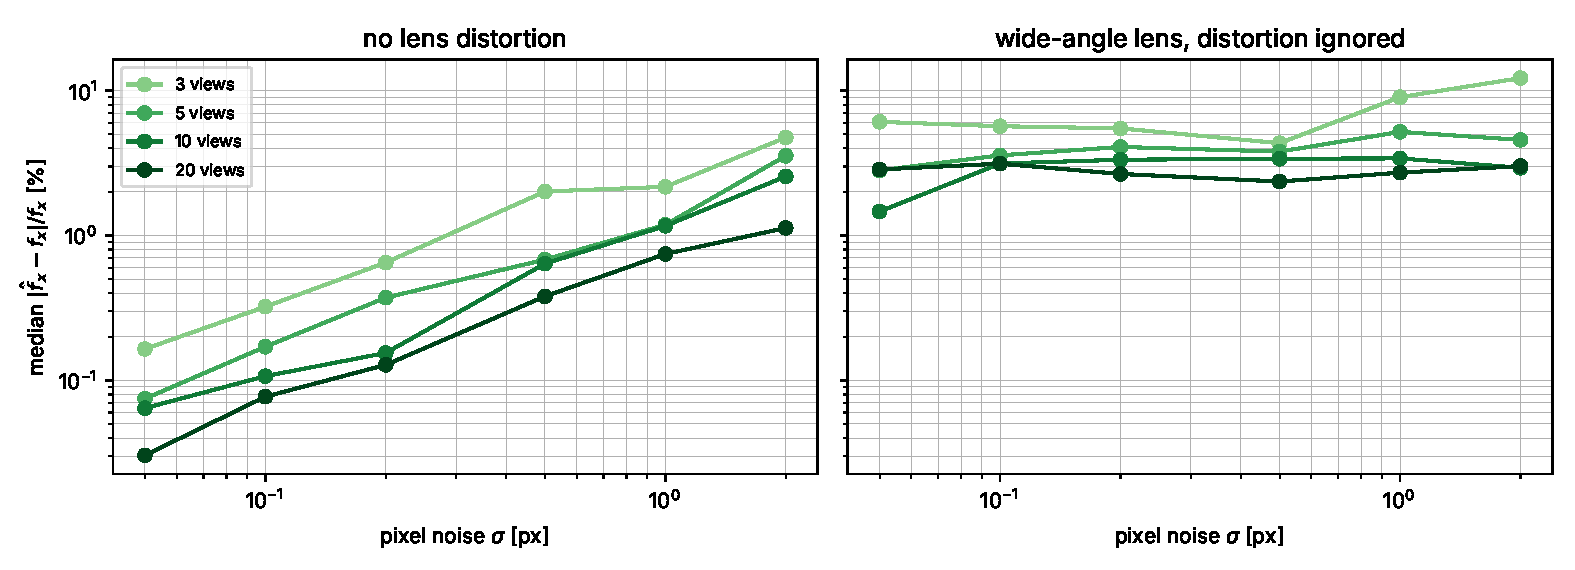
\includegraphics[width=\linewidth]{figures/ch03_zhang.pdf}
\caption{Median relative error on $f_x$ of the linear step of Zhang's
method (40 random trials per point). Left: ideal lens; the error scales
linearly with pixel noise and decreases with the number of views. Right:
the wide-angle lens of \cref{fig:distortion}, whose distortion the
linear step ignores: a bias of a few percent remains however many views
and however little noise.}
\label{fig:zhang}
\end{figure}

\section{Stereo and depth sensors}

\begin{definition}{Rectified stereo pair}{stereo}
Two identical undistorted pinhole cameras whose frames differ by a pure
translation of $b>0$ (the \emph{baseline}) along the left camera's $x$
axis. A point $\vect{q}=(X,Y,Z)$ in the left frame is measured as
\[
\z=(u_l,v,u_r),\quad u_l=f_x\frac{X}{Z}+c_x,\quad
v=f_y\frac{Y}{Z}+c_y,\quad u_r=f_x\frac{X-b}{Z}+c_x .
\]
Real stereo cameras are \emph{rectified} to this form by warping both
images after calibration, so that matching points share the same row
$v$.
\end{definition}

\begin{proposition}{Depth from disparity}{disparity}
The disparity $\delta=u_l-u_r$ equals $f_xb/Z$, so $Z=f_xb/\delta$. If
$\delta$ is measured with standard deviation $\sigma_\delta$, the first-
order standard deviation of the depth is
\begin{equation}\label{eq:depthstd}
\sigma_Z=\frac{Z^2}{f_x\,b}\,\sigma_\delta .
\end{equation}
\end{proposition}

\begin{proof}
Subtract the expressions of $u_l$ and $u_r$:
$\delta=f_x(X-(X-b))/Z=f_xb/Z$. Then $\mathrm{d}Z/\mathrm{d}\delta=
-f_xb/\delta^2=-Z^2/(f_xb)$, and first-order propagation gives
\eqref{eq:depthstd}.
\end{proof}

\begin{inwords}
Depth error grows with the \emph{square} of the distance: a stereo
camera that is precise to a centimetre at one metre is precise to a
metre at ten. A wider baseline helps linearly, but makes near objects
harder to match. \Cref{fig:stereo} shows the trade-off; the Monte Carlo
dots also show that at long range the depth distribution becomes skewed
(depth is the reciprocal of a Gaussian disparity), which is one reason
modern systems parametrise far points by \emph{inverse} depth.
\end{inwords}

\begin{figure}[ht]
\centering
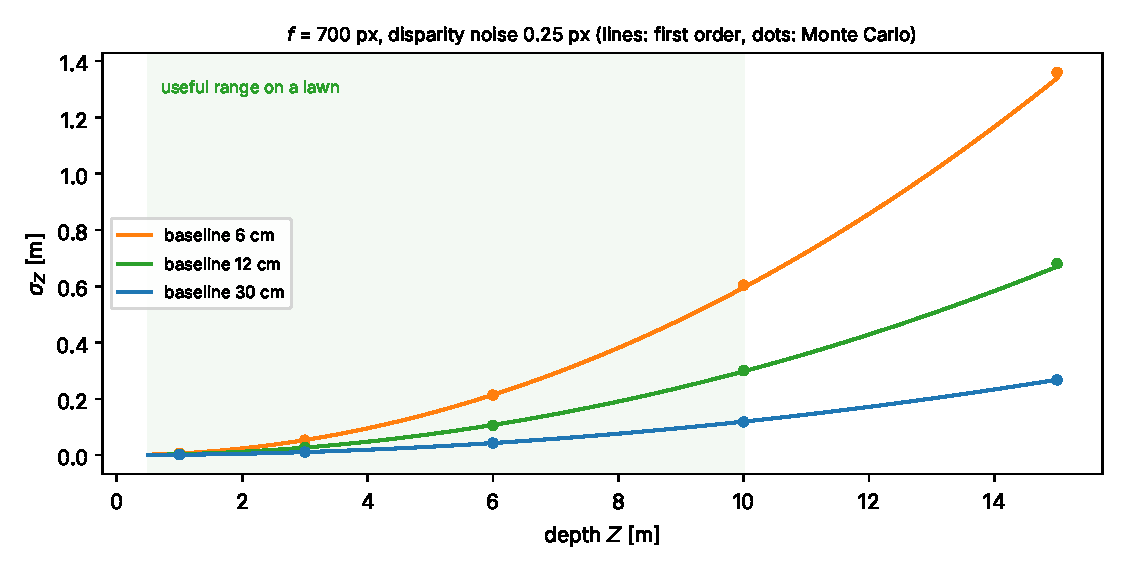
\includegraphics[width=0.85\linewidth]{figures/ch03_stereo.pdf}
\caption{Depth uncertainty of a rectified stereo pair with $f=700$\,px
and $0.25$\,px disparity noise, for three baselines. Lines:
\eqref{eq:depthstd}; dots: Monte Carlo triangulation.}
\label{fig:stereo}
\end{figure}

RGB-D cameras measure depth directly, by projecting an infrared pattern
(structured light) or timing light pulses (time of flight). They are
excellent indoors and, for the mower, nearly useless: sunlight swamps
their infrared signal.

\begin{mower}
What this chapter says about the camera to put on the mower:
\begin{itemize}[nosep]
\item \emph{Global shutter.} A rolling-shutter sensor exposes rows at
  different times; with the vibration of the cutting deck and a moving
  platform this distorts geometry in ways the pinhole model cannot
  express.
\item \emph{Stereo, baseline 10--20\,cm.} It removes the monocular scale
  gauge and, by \eqref{eq:depthstd}, gives useful depth to about 10\,m;
  Exercise~\ref{ex:3base} sizes it.
\item \emph{Wide field of view, mounted high and tilted down.} A wide
  view keeps far, stable features (fences, trees, buildings) in sight
  while the mower turns; the downward tilt keeps nearby ground in view
  for motion estimation. Calibrate with the distortion model that fits
  the lens.
\item \emph{Fixed exposure or controlled auto-exposure}, since the scene
  alternates between bright lawn and deep shade under trees.
\end{itemize}
\end{mower}

\begin{practice}[\code{vslam/camera.py}, \code{vslam/calib.py},
  \code{examples/ch03\_cameras.py}, \code{notebooks/ch03\_cameras.ipynb}]
\begin{center}
\begin{tabular}{@{}ll@{}}
\toprule
Code & Formula\\
\midrule
\code{perspective} & $\pi$ and $\Pi$\\
\code{PinholeCamera.distort}, \code{distort\_jacobian} &
  \cref{def:distortion}, \cref{prop:undistort}\\
\code{PinholeCamera.undistort}, \code{unproject} &
  Newton (\cref{prop:undistort}), \cref{lem:ray}\\
\code{PinholeCamera.project\_world} & \cref{prop:projjac}\\
\code{StereoCamera} & \cref{def:stereo}, \cref{prop:disparity}\\
\code{calib.homography\_dlt} & \cref{prop:dlt} with normalisation\\
\code{calib.zhang\_intrinsics} & \cref{thm:zhang}, \cref{prop:kfromb}\\
\code{calib.zhang\_extrinsics}, \code{nearest\_rotation} &
  \cref{lem:boardH}, \cref{lem:nearestrot}\\
\bottomrule
\end{tabular}
\end{center}
The tests check every Jacobian against finite differences,
$d^{-1}\circ d=\mathrm{id}$, the agreement of \code{project\_world} with
the projection matrix \eqref{eq:projmat}, and exact recovery of $K$ and
of every board pose by Zhang's method from noise-free views (three views,
two with zero skew). \code{look\_at(eye, target)} builds camera poses;
\code{calib.synthetic\_views} simulates checkerboard images.

The script produces \cref{fig:distortion,fig:zhang,fig:stereo}. The
notebook goes further: it calibrates a simulated wide-angle camera,
displays the reprojection residuals of the linear estimate (about
3\,px, systematic, thirty times the pixel noise), and checks
\eqref{eq:projjac} numerically.
\end{practice}

\section*{Further reading and C++ pointers}
\addcontentsline{toc}{section}{Further reading and C++ pointers}

Hartley and Zisserman, chapters~6 and~7 (cameras) and~4 (homographies,
the DLT and normalisation). Z.~Zhang, ``A flexible new technique for
camera calibration'', \emph{IEEE TPAMI} 22(11), 2000. In practice:
OpenCV's \code{calibrateCamera} and \code{stereoCalibrate} for
intrinsics and stereo, and \code{Kalibr} for the camera--IMU calibration
needed in Part~IV.

\FloatBarrier
\section*{Exercises}
\addcontentsline{toc}{section}{Exercises}

\begin{enumerate}[label=\textbf{3.\arabic*},ref=3.\arabic*]
\item\label{ex:3centre} Show that the camera centre $\tilde{\vect{c}}=
  (\vect{c},1)$ spans the null space of $P$ in \eqref{eq:projmat}, and
  that $P$ has 11 degrees of freedom.
\item\label{ex:3rot} \emph{Turning on the spot.} Two images are taken
  from the same centre, the second camera rotated by $R=R_{c_1c_2}\T$
  relative to the first. Show that corresponding pixels satisfy
  $\tilde{\vect{u}}_2\sim KRK^{-1}\tilde{\vect{u}}_1$ whatever the depth
  of the point. What does this imply for a mower that turns on the spot?
\item\label{ex:3skew} Show that $B_{12}=-s/(f_x^2f_y)$, so that
  $B_{12}=0$ exactly when the skew vanishes.
\item\label{ex:3base} With $f_x=700$\,px and $\sigma_\delta=0.25$\,px,
  what baseline gives $\sigma_Z\le5$\,cm at $5$\,m? At $10$\,m?
\end{enumerate}

\subsection*{Solutions}

\textbf{3.1.} $P\tilde{\vect{c}}=K(R_{cw}\vect{c}+\vect{t}_{cw})$, and
$R_{cw}\vect{c}+\vect{t}_{cw}$ is the centre expressed in its own camera
frame, i.e.\ $\vect0$. $P$ has rank 3 (its left $3\times3$ block
$KR_{cw}$ is invertible), so its null space is one-dimensional and is
spanned by $\tilde{\vect{c}}$. Degrees of freedom: 5 for $K$, 3 for
$R_{cw}$, 3 for $\vect{t}_{cw}$, total 11; equivalently 12 entries
minus one for the overall scale, since $P$ acts on $\mathbb{P}^3$.

\textbf{3.2.} With a common centre $\vect{c}$, the two camera-frame
coordinates of a point are $\vect{q}_i=R_{c_iw}(\p_w-\vect{c})$, so
$\vect{q}_2=R_{c_2w}R_{c_1w}\T\vect{q}_1=R_{c_1c_2}\T\vect{q}_1=R
\vect{q}_1$. Then $\tilde{\vect{u}}_2\sim K\vect{q}_2=KR\vect{q}_1\sim
KRK^{-1}\tilde{\vect{u}}_1$, using $\vect{q}_1\sim K^{-1}\tilde{\vect{u}}
_1$. The relation holds for every point, near or far, so the two images
carry no information about depth or structure: they are related by one
homography. A mower turning on the spot sees its rotation very well
(every pixel moves) but cannot triangulate anything new during the turn;
Chapter~6 shows this is a degenerate configuration for two-view
geometry, and the front-end must detect it.

\textbf{3.3.} $K^{-1}=\begin{pmatrix}1/f_x&-s/(f_xf_y)&(sc_y-c_xf_y)/
(f_xf_y)\\0&1/f_y&-c_y/f_y\\0&0&1\end{pmatrix}$ (check $KK^{-1}=I$).
$B=K^{-\mathsf T}K^{-1}$ has $B_{12}$ equal to the inner product of the
first two columns of $K^{-1}$, namely $\frac1{f_x}\cdot\bigl(-\frac{s}
{f_xf_y}\bigr)+0+0=-\frac{s}{f_x^2f_y}$.

\textbf{3.4.} From \eqref{eq:depthstd}, $b\ge Z^2\sigma_\delta/(f_x
\sigma_Z)$. At $5$\,m: $25\times0.25/(700\times0.05)\approx0.18$\,m. At
$10$\,m: four times more, $0.71$\,m, too wide for a mower; beyond a few
metres depth must come from motion (multi-view triangulation over a
long baseline travelled by the mower) rather than from the stereo rig
alone.
